\chapter{Background}\label{sec:background}

% Purpose: Provide the necessary context for your research. This may include the problem you are solving, why it's important, and the related state-of-the-art and background information in order to understand the work developed in the thesis.
% 
% Content:
%     + Fundamental concepts or theories
%     + Terminology definitions
%     + High-level overview of the problem domain
%     + Historical context if applicable
%
% Audience: Assumes the reader may not be an expert in the specific area of your research but has some knowledge of the broader field.

This section is dedicated to the background information needed to understand the work developed in the thesis. It provides the necessary context for the research, including the problem being solved, why it's important, and the related state-of-the-art and background information. It also includes fundamental concepts and theories, terminology definitions, and a high-level overview of the problem domain. It serves as a primer to the rest of the report, providing the necessary context for the research and is intended for readers who may not be experts in the specific area of the research but have some knowledge of the broader field.

\section{SSH and OpenSSH Implementation}\label{sec:background:ssh}

    \subsection{Basics of the Secure Shell Protocol (SSH)}
    
    The Secure Shell Protocol, commonly known as \acrshort{ssh}, is designed to facilitate secure remote login and other secure network services over insecure networks. \acrshort{ssh} has been design since its inception with security in mind, as a successor of the Telnet protocol, which is not secure, and other \say{unsecured remote shell protocols such as rlogin, rsh and rexec} \cite{SSHkex22}. 
    
    \subsubsection{SSH design and origin}
    As stated by the authors of the \citetitle{SSHReport18}, \say{The founder of SSH, Tatu Ylönen, designed the first version of the SSH protocol after a password-sniffing attack at his university network. Tatu released his implementation as freeware in July 1995, and the tool quickly gained in popularity. Towards the end of 1995, the SSH user base had grown to 20,000 users in fifty countries. By 2000, there were an estimated 2,000,000 users of the protocol. Today, more than 95\% of the servers used to power the Internet have SSH installed in them. The SSH protocol is truly one of the cornerstones of a safe Internet.} \cite{SSHReport18}.

    \acrshort{ssh} is defined in \citetitle{RFC4251} \cite{RFC4251}. It is divided into three major components:

    \begin{itemize}
        \item \textbf{Transport Layer Protocol:} This provides server authentication, confidentiality, and integrity. It can also optionally provide compression. Typically, the transport layer runs over a TCP/IP connection but can also be used on top of any other reliable data stream.
        \item \textbf{User Authentication Protocol:} Running over the transport layer, this protocol authenticates the client-side user to the server. Multiple methods of authentication such as password and public key are supported.
        \item \textbf{Connection Protocol:} This multiplexes the encrypted tunnel established by the preceding layers into several logical channels. Channels can be used for various purposes, such as setting up secure interactive shell sessions or tunneling arbitrary TCP/IP ports.
    \end{itemize}

    \say{The client sends a service request once a secure transport layer connection has been established. A second service request is sent
    after user authentication is complete. This allows new protocols to be defined and coexist with the protocols listed above} \cite{RFC4251}.

    \subsubsection{SSH keys}\label{sec:background:ssh:ssh_keys}
    For the purposes of this Masterarbeit, a comprehensive understanding of SSH's key exchange and encryption mechanism is important. As outlined in SSHKex \cite{SSHkex22}, the SSH protocol utilizes a key exchange procedure that culminates in a derived master key \( K \) and a hash value \( h \). These components are pivotal for encrypting client-server communications and identifying sessions.

    During the key exchange process, Diffie-Hellman is employed to negotiate an ephemeral shared key between the client and the server \cite{RFC4251} \cite{StackExchangeSSHuseRASandDH23}. This ephemeral key is then signed by the server using either RSA, DSA, or another suitable signature algorithm (see \ref{subsubsec:background:ssh:hashing}). The signed key confirms to the client that the negotiated key is indeed from the intended server and not an imposter or a middleman, thereby preventing man-in-the-middle (MITM) attacks.

    In addition, the host key of the server is used to sign the Diffie-Hellman parameters. This key is not to be confused with the client key listed in the server's \texttt{authorized\_keys} file, which is used later for client authentication.

    The key exchange process results in multiple session keys computed for various purposes:

    \begin{itemize}
        \item \textbf{Initialization Vectors:} Key A and Key B are designated for initialization vectors from the client to the server and vice versa.
        \item \textbf{Encryption Keys:} Key C and Key D act as encryption keys for client-to-server and server-to-client communications, respectively.
        \item \textbf{Integrity Keys:} Key E and Key F are utilized to preserve the integrity of data transmitted between the client and server.
    \end{itemize}

    This approach provides forward secrecy: if the private key is stolen, it does not compromise the encryption of old sessions. This is because the Diffie-Hellman parameters are ephemeral and discarded once they are no longer needed. Therefore, the only long-lasting keypair is used for authentication purposes.

    \subsubsection{SSH key encryption}
    These keys are computed using hash functions that take the master key \textit{K} and a hash value \textit{h}, a unique letter (A, B, C, D, E, or F), and the session ID as inputs. This is summarized in \citetitle{OpenSSHUnderHood07}:
    \say{
        The equations used for deriving the above vectors and keys are taken from RFC 4253 \cite{RFC4253}. In the following, the $||$ symbol stands for concatenation, K is encoded as mpint, $"A"$ as byte and $session_id$ as raw data. Any letter, such as the $"A"$ (in quotation marks) means the single character A, or ASCII 65.
        \begin{itemize}
            \item Initial IV client to server: $HASH(K || H || "A" || session_id)$.
            \item Initial IV server to client: $HASH(K || H || "B" || session_id)$.
            \item Encryption key client to server: $HASH(K || H || "C" || session_id)$.
            \item Encryption key server to client: $HASH(K || H || "D" || session_id)$.
            \item Integrity key client to server: $HASH(K || H || "E" || session_id)$.
            \item Integrity key server to client: $HASH(K || H || "F" || session_id)$.
        \end{itemize}
    } \cite{OpenSSHUnderHood07}. Details about the hash function are given in the next section.
    
    The most interesting keys are the encryption keys, as they are used to encrypt the communication between the client and the server. The other keys are used for integrity checks and initialization vectors. Decrypting encrypted SSH communication necessitates either to retreive these session keys and variables so as to recompute the keys, or to retreive those keys directly, which is the focus of this Masterarbeit. 

    \subsection{OpenSSH Implementation}
    OpenSSH (OpenBSD Secure Shell) is an open-source implementation written in C of the SSH protocol suite, and it is the most widely used SSH implementation \cite{OpenSSHUnderHood07}. It is the default SSH implementation on most Linux distributions, and it is also available for Windows. OpenSSH is used for a wide range of purposes, including remote command-line login and remote command execution. It is also used for port forwarding, tunneling, and transferring files via SCP and SFTP either manually or via automated processes, such as backup systems, configuration management tools, and automated software deployment tools. 

    \subsubsection{OpenSSH components}
    OpenSSH is composed of several tools and daemons, including client and server components \cite{PortableOpenSSHGitHub}:
    \begin{itemize}
        \item \textbf{ssh:} The basic client program that allows to log into and execute commands on a remote machine.
        \item \textbf{sftp:} An interactive file transfer program that uses SSH to secure the connection.
        \item \textbf{sshd:} This is the SSH daemon that runs on the server. This is used for connecting to a remote machine when using the SSH client from another system.
        \item \textbf{ssh-agent:} The program that holds private keys in memory, so one doesn't have to enter ones passphrase every time.
        \item \textbf{ssh-add:} A program for adding RSA or DSA identities to the authentication agent.
        \item \textbf{ssh-keygen:} A utility for creating and managing SSH keys.
        \item \textbf{ssh-keyscan:} A utility for gathering public SSH host keys from a number of hosts.
        \item \textbf{ssh-keychk:} A utility for checking the validity of SSH keys.
        \item Several other tools to support the SSH protocol and the OpenSSH implementation.
    \end{itemize}

    \subsubsection{OpenSSH hashing}\label{subsubsec:background:ssh:hashing}
    OpenSSH employs a variety of hash functions and algorithms to secure data, most commonly using SHA1. However, SHA1 is increasingly seen as weak due to its vulnerability to collision attacks \cite{OpenSSHUnderHood07}. In light of this, the contemporary standard leans towards SHA512. The hash functions are used alongside cipher algorithms like \say{Advance Encryption Standard (AES) Cipher Block Chaining (CBC), AES Counter (AES-CTR), and ChaCha20} \cite{SmartKex22}. The Message Authentication Code (MAC) typically uses either MD5 or SHA1 hash algorithms in combination with a secret key. Since cybersecurity and cryptography are constantly evolving, so do \acrshort{ssh} and OpenSSH. Depending on the version \cite{OpenSSHUnderHood07}, the available hash options include:
    
    \begin{itemize}
        \item \textbf{ssh-dss:} \textit{(disabled at run-time since OpenSSH 7.0 released in 2015)} SSH-1 version using Digital Signature Algorithm (DSA) from the Digital Signature Standard (DSS). Originally popular but phased out due to vulnerabilities to collision attacks for DSA Key in a 1024-bit modulus. As stated by \citetitle{RFC9142}: \say{These attacks are still computationally very difficult to perform, but it is desirable that any key exchange using SHA-1 be phased out as soon as possible} \cite{RFC9142} \cite{OpenSSHReleaseNotes7-0}.
        
        \item \textbf{ssh-rsa:} \textit{(disabled at run-time since OpenSSH 8.8 released in 2021)} It refers to the use of RSA (Rivest-Shamir-Adleman) encryption algorithm. In the context of SSH-1, this version had to be replaced due to the related to key size issue similar to DSS: \say{RSA 1024-bit keys have approximately 80 bits of security strength}... \say{which may not be sufficient for most users.} \cite{RFC9142} \cite{OpenSSHReleaseNotes8-8}.
        
        \item \textbf{ecdsa-sha2-nistp256:} \textit{(since OpenSSH 5.7 released in 2011)} Uses the SHA-2 family for hashing and the NIST P-256 curve. It is considered secure and efficient, with an \acrfull{ess} of 128 bits \cite{RFC9142} \cite{OpenSSHReleaseNotes5-7}.
        
        \item \textbf{ecdsa-sha2-nistp384:} \textit{(since OpenSSH 5.7)} Utilizes the SHA-2 family and the larger NIST P-384 curve for additional security at the cost of performance. It has an \acrshort{ess} of 192 bits \cite{RFC9142} \cite{OpenSSHReleaseNotes5-7}.
        
        \item \textbf{ecdsa-sha2-nistp521:} \textit{(since OpenSSH 5.7)} Employs SHA-2 and the even larger NIST P-521 curve for maximal security with an \acrshort{ess} of 256 bits \cite{RFC9142}. It is less commonly used due to performance considerations \cite{OpenSSHReleaseNotes5-7}. 
        
        \item \textbf{ssh-ed25519:} \textit{(since OpenSSH 6.5 released in 2014)} Known for high security and performance efficiency; employs the Ed25519 elliptic curve with an \acrshort{ess} of 128 bits \cite{RFC9142} which is similar to $ecdsa-sha2-nistp256$, and has been more prevalent following the 2013 suspicions of NSA backdoors in NIST curves \cite{Adamantiadis2013} following the Snowden revelations \cite{NSAFoilSafeguards2013} \cite{GuardianEncryption2013} \cite{OpenSSHReleaseNotes6-5}.
        
        \item \textbf{rsa-sha2-256:} \textit{(since OpenSSH 7.2 released in 2016)} An upgrade from ssh-rsa, using SHA-256 (with \acrshort{ess} of 128 bits) for hashing to improve security without major performance hits \cite{OpenSSHReleaseNotes7-2}.
         
        \item \textbf{rsa-sha2-512:} \textit{(since OpenSSH 7.2)} Similar to $rsa-sha2-256$ but employs SHA-512 for even stronger security, albeit with some performance cost \cite{OpenSSHReleaseNotes7-2}.
        
        \item \textbf{ecdsa-sk:} \textit{(since OpenSSH 8.2 released in 2020)} Security Key-enabled, uses NIST curves and is geared towards modern hardware-based authentication \cite{OpenSSHReleaseNotes8-2}.
        
        \item \textbf{ed25519-sk:} \textit{(since OpenSSH 8.2)} Similar to ssh-ed25519 but integrates hardware-based Security Keys for an additional layer of security \cite{OpenSSHReleaseNotes8-2}.
        
        \item \textbf{NTRU Prime-x25519:} \textit{(since OpenSSH 9.0)} A new, highly secure algorithm focused on post-quantum cryptography, providing future-proof security \cite{NTRUPostQuantum17} \cite{OpenSSHReleaseNotes9-0}.
    \end{itemize}
    
    These hashes have fixed lengths such that key lengths range between 12 and 64 bytes \cite{SmartKex22}. Since high-quality random number generation is crucial to ensure that thoses keys are secure and difficult to predict, it can thus be assumed that thoses key have a high entropy \cite{McLaren2019}. This is a crucial assumption as it is the basis for the use of both brute force and machine learning algorithms to predict the presence and location of SSH keys in memory dumps.

    The keys generated by these hash functions are pseudo-random numbers stored in the system's RAM. Following the Kerckhoffs' principle: that \say{a cryptosystem should be secure, even if everything about the system, except the key, is public knowledge}, the code for the OpenSSH implementation is open-source and available on GitHub \cite{PortableOpenSSHGitHub}. This allows for the analysis of the code and the identification of the memory structures where the keys are stored.

    \subsection{The state of SSH security}
    Since its origins, SSH has been developed with cybersecurity in mind, and is generally considered a secure method for remote login and other secure network services over an insecure network. However, as with any technology, it can be exploited if not configured or managed correctly. The protocol is used by system administrators to manage remote systems, and it is also used by automated processes to transfer data and perform other tasks. This makes SSH a valuable target for attackers. In fact, SSH has been a popular target for cyber-attacks. Due to being so prevalent, it is often used by threat actors either as a vector for initial access, as a means to move laterally across a network or as a covered exit for exfiltration of sensitive data \cite{APTTactics19}. The encrypted nature of its communications makes it an attractive option for attackers, as it can be difficult to detect malicious activity.
    
    \subsubsection{SSH security issues}
    Here are some cases where SSH can involved in cyber-attacks, although it's important to note that SSH itself is not inherently insecure:
    \begin{itemize}
        \item \textbf{SSH Brute-Force Attacks:} One of the most common types of attacks involving SSH is a brute-force attack, where an attacker tries to gain access by repeatedly attempting to login with different username-password combinations. These attacks are not sophisticated but can be effective if strong authentication measures are not in place. For instance, the botnet \textit{Chabulo} was used to launch a large-scale brute-force attack \say{through compromised SSH servers and IoT devices} in 2018 \cite{SSHReport18}. 
        \item \textbf{SSH Key Theft:} In some advanced attacks, threat actors have stolen SSH keys to move laterally across a network after initial entry. This allows them to authenticate as a legitimate user and can make detection much more challenging. It can \say{ occurs when users have their SSH password or unencrypted keys stolen through a variety of methods (sniffed via a key-logging console program, shoulder-surfed via bad security awareness, poor key management practices, etc.).} \cite{SSHIdentityTheft05}.
        \item \textbf{Man-in-the-Middle Attacks:} Although SSH is designed to be secure, it can be susceptible to man-in-the-middle attacks if proper verification of SSH keys is not done during the initial connection setup \cite{OpenSSHUnderHood07}.
        \item \textbf{Misconfiguration:} As with any technology, misconfiguration can lead to security issues. For example, leaving default passwords, using weak encryption algorithms, or enabling root login can all make an SSH-enabled system vulnerable \cite{SSHBotnetInfect21}.
    \end{itemize}

    \subsubsection{SSH vulnerabilities}
    In cybersecurity, it is generally considered that any system that is connected to the Internet will be attacked at some point. Similarly, it is a common saying that no system is 100\% secure. This is true for SSH as well. Although it is a secure protocol, it can be exploited if not configured or managed correctly. 
    
    Some vulnerabilities have also been discovered in the protocol itself, although these are rare.
    \begin{itemize}
        \item \textbf{SSH-1 Vulnerabilities:} A series of vulnerabilities in the first implementation of SSH were discovered from 1998 to 2001, with its subsequent fixes leading to unauthorized content insertion and arbitrary code execution. SSH-1 had many design flows and is now considered obsolete. \cite{CoreSecurity23}, \cite{SSH1Vulnerability01}. 
        \item \textbf{CBC Plaintext Recovery:} A theoretical vulnerability discovered in 2008 affecting all versions of SSH, allowing the recovery of up to 32 bits of plaintext from CBC-encrypted ciphertext \cite{USCERT2011}.
        \item \textbf{Suspected Decryption by NSA:} Leaked information in 2014 suggested that the NSA might be able to decrypt some SSH traffic, although the protocol itself was not confirmed to be compromised \cite{Spiegel14}.
    \end{itemize}
    
    \subsubsection{SSH and cyber-attacks}
    SSH has been used in many high-profile cyber-attacks and malwares, including the following:
    \begin{itemize}
        \item \textbf{Operation Windigo:} This was a large-scale campaign that infected over 25,000 UNIX servers. SSH was one of the vectors used for maintaining control over compromised servers. A report by ESET mentions that the  OpenSSH backdoor Linux/Ebury was first discovered in 2011 as a component of the aforementioned operation. \say{This operation has been ongoing since at least 2011 and has affected high profile servers and companies, including cPanel - the company behind the famous web hosting control panel - and Linux Foundation's kernel.org - the main repository of source code for the Linux kernel} \cite{ESETWindigo14}. 
        \item \textbf{Linux/Hydra:} Initially unleashed in 2008, this malware is a fast login cracker that targets a range of popular protocols including SSH. Hence, SSH is one of its primary vectors to gain initial access to Internet of Things (IoT) devices. Once a device is infected by Linux/Hydra, it joins an IRC channel and initiates a SYN Flood attack \cite{ClassificationMalware21}.
        \item \textbf{Psyb0t:} Discovered in early 2009, Psyb0t is an IRC-controlled malware specifically designed to target devices with MIPS architecture, such as routers and modems. Notably, it was responsible for orchestrating a DDoS attack against the DroneBL service, infecting up to 100,000 devices for this purpose. The malware is equipped to conduct UDP and ICMP flood attacks and employs a brute-force attack mechanism against Telnet and SSH ports. Remarkably, it uses a pre-configured list of 6,000 usernames and 13,000 passwords to perform these attacks \cite{ClassificationMalware21}.
        \item \textbf{Chuck Noris:} Similar to Psyb0t in its objectives and methods, Chuck Noris targets routers and DSL modems, focusing on SoHo (small office/home office) devices. However, unlike Psyb0t, which uses ICMP flood attacks, Chuck Noris deploys ACK flood attacks. The malware carries out brute-force attacks on Telnet and SSH open ports, drawing parallels to the tactics employed by Psyb0t but with the specific variation in flooding techniques \cite{ClassificationMalware21}.
    \end{itemize}

    It's worth noting that in many of these cases, SSH was not the initial attack vector but was used at some stage in the attack lifecycle. Properly configured and managed SSH is still considered a secure and robust protocol for remote access and data transfer. In all those situations, a tool monitoring the SSH traffic could have detected the malicious activities and prevented the attack.

    \subsection{The Imperative of SSH Honeypots in Cybersecurity Monitoring}
    SH (Secure Shell) has become an indispensable protocol for secure communication but can also conceil malicous agents. This reality underscores the urgency for robust monitoring mechanisms capable of identifying suspicious activities in real-time. Among various countermeasures, SSH honeypots have emerged as a particularly effective tool for monitoring and gathering intelligence on potential threats. 

    An SSH honeypot is a decoy server or service that mimics legitimate SSH services. The primary aim is to attract cybercriminals and study their tactics, thereby offering an active form of surveillance and data collection. Unlike traditional intrusion detection systems, honeypots do not merely identify an attack; they engage the attacker in a controlled environment, enabling detailed observation and logging of the intruder's actions. This allows for the collection of valuable information, such as the attacker's IP address, the tools used, and the techniques employed. This data can then be used to enhance security measures and develop more robust countermeasures \cite{ClassificationMalware21}. 

    SSH honeypots serve as an invaluable asset in the cybersecurity arsenal, providing not just a reactive but a proactive measure against evolving cyber threats. They can collect actionable intelligence on new hacking methods, malware, and exploitation scripts. This information can be crucial for proactively securing actual production environments. The data collected can also be used to trace back to the origin of the attack, facilitating legal pursuits against the perpetrators. By diverting attackers to decoy servers, honeypots also protect real assets from being targeted, saving both computational resources and administrative effort needed for post-incident recovery.

    Popular SSH honeypots include Kippo, Cowrie, and HoneySSH.  Cowrie is a fork of Kippo, with additional features such as logging of attacker's keystrokes and file transfer. 

    \begin{itemize}
        \item \textbf{Kippo:} Kippo is a medium-interaction honeypot that logs the attacker's shell interaction. It specializes in capturing brute force and Telnet-based attacks \cite{ClassificationMalware21}.
        
        \item \textbf{Cowrie:} Serving as Kippo's successor, Cowrie emulates various protocols including SSH, SFTP, and SCP. It logs events in JSON format, making it particularly useful for detecting brute force and Telnet-based attacks, as well as spoofing attacks \cite{ClassificationMalware21}.
        
        \item \textbf{IoTPOT:} This IoT-focused honeypot supports multiple CPU architectures and can detect a variety of attacks including brute force, DoS, and sniffing attacks on Telnet, SSH, and HTTP ports \cite{ClassificationMalware21}.
        
        \item \textbf{HoneySSH:} HoneySSH is a low-interaction honeypot that emulates an SSH server and logs the attacker's IP address, username, and password \cite{honeyssh17}.
        
        \item \textbf{Sarracenia (SSHKex):} Introduced in 2018, Sarracenia is a high-interaction SSH honeypot that has been enhanced by SSHKex. Instead of \say{requiring the VM to be paused for every incoming or outgoing packet, which degrades the server performance} \cite{SSHkex22}, SSHKex allows for the extraction of derived SSH session keys. This reduces the performance degradation significantly, as the VM is paused less frequently \cite{SSHkex22} \cite{SarraceniaSSHHoneypot18}.
    \end{itemize}

    These honeypots are useful tools for gathering intelligence on potential threats. However, they are not without their limitations.

    \subsection{Research context and motivation for this Masterarbeit}

    Security and malware detection are active areas of research, with SSH honeypots being a particularly promising tool for gathering intelligence on potential threats. However, they are not without their limitations. For instance, they are not able to perfectly mimic a real system, such that attackers might be able to detect them \citetitle{SSHHoneypotEffectiveness23}. 
    
    As explained in \citetitle{SSHHoneypotEffectiveness23}: \say{As attackers become more sophisticated with their ransomware and malware campaigns, there is a significant need for security researchers to assist the greater community by running vulnerable honeypot machines to collect malicious software}. \citeauthor{SSHHoneypotEffectiveness23} explain that \say{the ability to collect meaningful malware from attackers depends on how the attackers receive the honeypot. Most attackers fingerprint targets before they launch their attack, so it would be very beneficial for security researchers to understand how to hide honeypots from fingerprinting and trick the attackers into depositing malware.} They conclude that \say{What is certain is that if a cautious attacker believes they are in a honeypot, they will leave without depositing malware onto the system, which reduces the effectiveness of the honeypot for security research.} We can extrapolate this conclusion to SSH honeypots, which are also vulnerable to fingerprinting and detection by attackers. 
    
    Hence, the need for more advanced SSH honeypots-inspired tools that can leverage data forensic and machine learning techniques so as to be able to use directly a real server as a honeypot, without the need to emulate a system. The current master's thesis is aligned with this ongoing research (see \ref{chapter:related_work}), further enhancing the state of SSH honeypots. It aims to develop algorithms, proof of concepts and tools that can extract SSH keys from memory dumps of a real server, and use them to decrypt SSH traffic. This could lead to the developement of new tools for SSH monitoring, as discussed in the future work section \ref{conclusion:sec:future_work}.

\section{Graph-based memory modelization}\label{sec:background:graph}

    In the following section, we present important concepts that will be used for the memory modelization of the heap dump.

    Because the dataset used is composed of RAW heap dump files from OpenSSH, it is a critical aspect to understand how memory works at a low level point of view. This section aims to provide an in-depth understanding of how memory is managed in C, the language used in the OpenSSH implementation of SSH, for a \textit{linux-x86\_64} architecture. We will explore the fundamental concepts of memory management, including the heap and the stack, memory allocation, and the role of pointers. These concepts will serve later as the foundation for our graph-based approach to memory modelization.

    This section will also introduce many graph theory and \acrfull{kg} concepts. We will explore the fundamentals of graph theory, including the definition of a graph, its components, and its properties. We will also discuss the concept of a \acrfull{kg}, which is a type of graph that stores information in the form of nodes and edges, and its applications in the field of machine learning.

    \subsection{Defining memory concepts and modelization}
    Memory management in C is a complex task that requires a deep understanding of the language's features, the operating system's capabilities and the compiler used. In C, memory is primarily managed through two built-in functions: \texttt{malloc} (memory allocation) and \texttt{free} (memory deallocation). These functions operate on two primary types of memory: the heap and the stack.

    \begin{itemize}
        \item \textbf{Heap vs Stack:} The heap is used for dynamic memory allocation, where variables are allocated and freed at runtime. In contrast, the stack is used for static memory allocation, where variables are allocated and deallocated automatically. The stack is faster but has a limited size, while the heap is more flexible but requires manual management to prevent memory leaks.
        
        \item \textbf{Heap Dump:} A heap dump is a snapshot of the heap's state at a given time. It provides valuable information about the memory layout, active pointers, and data stored in the heap. Analyzing heap dumps can help in debugging memory-related issues and understanding the program's behavior.
        
        \item \textbf{Memory Addresses:} Each location in memory is identified by a unique memory address. These addresses are usually represented in hexadecimal notation. Note that the address $0x0$ is reserved for the \textit{NULL} pointer, which is used to indicate that a pointer does not point to any memory location.

        \item \textbf{Pointer:} A pointer is a variable that stores the memory address of another variable. It is used to indirectly access the value of the variable it points to. Pointers are used extensively in C, particularly for dynamic memory allocation.
        
        \item \textbf{Data Structure:} A data structure is a collection of data values, the relationships among them, and the functions or operations that can be applied to the data. In the context of C programming, data structures are declared using the keyword \texttt{struct} and are byte aligned. This means that the size of the data structure is always a multiple of the size of the largest member of the structure. Structures can be nested within each other, and pointers can be used to indirectly access the members of a structure. Data structures are often stored in the heap using \texttt{malloc}.
        
        \item \textbf{Malloc headers:} When \texttt{malloc} is called, it allocates a block of memory in the heap and returns a pointer to the first byte of the block. The heap manager keeps track of these allocations through metadata, often stored in headers preceding the allocated blocks. These headers contain information such as the size of the allocated block and whether it is free or occupied. Note that the pointer returned by malloc in C points to the first byte of the block of memory that has been allocated for your use, not to the malloc header. The malloc header, is managed internally by the memory allocator and is not exposed to the programmer, but is visible in the heap dump.
        
    \end{itemize}

    \subsubsection{Endianness}
    
    Endianness refers to the byte order used to represent multi-byte data types. In a \textit{little-endian} system, the least significant byte is stored first, while in a \textit{big-endian} system, the most significant byte is stored first. Knowing the endianness of the system is crucial for interpreting the content of memory \cite{InferenceEndianness17}.
    
    For instance, the hexadecimal value \textit{0x56343a198000} (taken from \textit{"HEAP\_START"} of \ref{lst:json-annotation-ex-1}) is represented as $550179058774$ ($\simeq 5.50e+11$) in decimal basis in a little-endian system, while it is represented as $94782313037824$ ($\simeq 9.48e+13$) in a big-endian system.

    \begin{minipage}{\dimexpr\linewidth-20pt}
        \paragraph{Little-Endian Conversion}
        The conversion of a hexadecimal number in \textit{little-endian} format to a decimal number is given by the following formula:
        \par % solve the underfull hbox warning
        
        \vspace{2em}  % Adds vertical space
        \begin{center}
            $
            \text{Decimal} = \sum_{i=0}^{N-1} \left( \text{HexDigit}_{i} \times 16^{i} \right)
            $
        \end{center}
        \vspace{1em}
    \end{minipage}
    
    \begin{minipage}{\dimexpr\linewidth-20pt}
        \paragraph{Big-Endian convertion}
        And the convertion of a hexadecimal number in \textit{big-endian} format to a decimal number is given by following formula:
        \par % solve the underfull hbox warning
        
        \vspace{2em}  % Adds vertical space
        \begin{center}
            $
            \text{Decimal} = \sum_{i=0}^{N-1} \left( \text{HexDigit}_{N-1-i} \times 16^{i} \right)
            $
        \end{center}
        \vspace{1em}
    \end{minipage}

    Here, $ \text{HexDigit}_{i} $ is the value of the \(i\)-th digit in the little-endian hexadecimal number, and \( N \) is the number of digits in the hexadecimal number. Note that $ \text{HexDigit}_{i} $ should be converted to its decimal equivalent ('A' becomes 10, 'B' becomes 11, etc.) before performing the calculation.

    These formulas will be used later to convert pointer addresses from hexadecimal to decimal format in \textit{mem2graph}.

    \subsubsection{The role of entropy in forensic analysis}

    Entropy plays a pivotal role in forensic analysis, particularly in the context of memory dumps analysis. It serves as a measure of uncertainty and randomness, which can be crucial for tasks such as endianness detection and identifying encrypted keys in memory.

    As defined by Shannon in the realm of information theory, it is a measure of the uncertainty or randomness associated with a set of possible outcomes \cite{InferenceEndianness17} \cite{TheoryOfCommunicationShannon1948}. In digital applications, when calculated using the logarithm to base 2, entropy represents the amount of bits of information in a message.

    \begin{minipage}{\dimexpr\linewidth-20pt}
        \paragraph{Entropy Formula}
        The entropy \( H \) of a message is calculated using the formula:
        \par % solve the underfull hbox warning
        
        \vspace{2em}  % Adds vertical space
        \begin{center}
            $
            H = - \sum_{i=1}^{n} p_i \log_2 p_i
            $
        \end{center}
        \vspace{1em}

        Where $ p_1, p_2, \ldots, p_n $ are the probabilities of the set of all possible messages \cite{InferenceEndianness17}.
    \end{minipage}

    Endianness, as presented before, refers to the byte order used to represent multi-byte data types in computer memory \cite{InferenceEndianness17}. It is necessary to know the endianness of the heap dump to correctly interpret the content of memory, and especially the addresses of potential pointers. In this context, entropy can be used to infer the endianness of a system by analyzing the distribution of byte values in a memory dump, as presented in \citetitle{InferenceEndianness17} \cite{InferenceEndianness17}.

    Entropy is also a key element for encryption key detection, since those should be random byte sequences with high entropy \cite{SmartKex22}. By examining 8-byte aligned data for high entropy, it is possible to detect potential keys in a heap dump. Techniques such as the calculation of discrete differences and logical operations can further refine this detection as described in \citetitle{SmartKex22} \cite{SmartKex22}.

    \subsection{Graphs and Knowledge Graphs}
    In this project, we (i.e. Clément Lahoche and the author) have built a program called \textit{mem2graph}, a generic tool developed in Rust for efficiency. It is used to convert a RAW memory dump into a graph representation. This graph is technically a directed Edge-labeled heterogeneous property graph, whose concepts are described later. As such, and while it is debatable whether or not \textit{mem2graph} can be seen as building Knowledge Graphs (KGs), it relies on many concepts from the domain, necessitating a proper introduction.

    \subsubsection{Defining Graph Theory concepts}
    Graph theory is a mathematical field concerned with the study of graphs. It has applications in various fields, including computer science, social sciences, or linguistics. Graphs are used to model pairwise relations between objects, and the study of graphs involves analyzing the properties of these relations. In a few words, a graph is just a collection of nodes and edges.
    
    A graph can be formally defined  as: \say{a pair \( G = (S, A) \) where:
    \begin{itemize}
        \item \( S \) is a finite set of vertices.
        \item \( A \) is a set of pairs of vertices \((s_i, s_j) \in S^2\).
    \end{itemize}
    Graphs can be either directed or undirected. In a directed graph, the pairs \((s_i, s_j)\) are ordered, representing arcs from \(s_i\) to \(s_j\). In an undirected graph, the pairs are unordered, representing edges between \(s_i\) and \(s_j\) } \cite{GraphTheorySolnon}. Let's introduce some vocabulary to describe graphs:

    \begin{itemize}
        \item \textbf{Node (or Vertex)}: A single entity in the graph, often represented as a circle.
        \item \textbf{Edge (or Arc)}: A connection between two nodes, often represented as a line or arrow.
        \item \textbf{Degree}: The number of edges connected to a node.
        \item \textbf{Path}: A sequence of edges that connect two nodes.
        \item \textbf{Cycle}: A path that starts and ends at the same node.
        every pair of nodes.
        \item \textbf{Order}: The number of vertices in the graph.
        \item \textbf{Adjascency}: Two nodes are adjacent if there is an edge between them.
        \item \textbf{Loop}: An edge that connects a node to itself.
        \item \textbf{Weight}: A value assigned to an edge.
        \item \textbf{Ancestors (parents) and Descendants (children)}: A node \(s_i\) is an ancestor of \(s_j\) if there is a path from \(s_i\) to \(s_j\). A node \(s_j\) is a descendant of \(s_i\) if there is a path from \(s_i\) to \(s_j\).
    \end{itemize}
    
    Various other terminologies and concepts exist in graph theory, but these are the most important ones for our purposes. For a more in-depth understanding of graph theory, the reader is encouraged to consult the work by \citeauthor{GraphTheorySolnon} as a quick introduction, \cite{GraphTheorySolnon} or a more in-depth one by \citeauthor{GraphTheoryIntro01} \cite{GraphTheoryIntro01}.

    \subsubsection{Graphs types}
    Graphs offer a flexible way to conceptualize, represent, and integrate diverse and incomplete data. Many graph models exist, each with its own advantages and disadvantages, as well as graph properties \footnote{Some parts of the following section are directly from a prior work for Seminar 5369S: Knowledge Graphs, written during summer 2023. As of the date of writting and to the best of my knowledge, this work has not been published, and as such, cannot be properly referenced.}. Those different types of graphs include:

    \begin{itemize}
        \item \textbf{Directed Edge-labelled Graphs (DEL):} The classic graph, set of nodes and edges that connect the nodes with in certain way. \acrshort{rdf} is a popular \acrshort{del} data model.
        \item \textbf{Heterogeneous Graphs:} Each node and edge is assigned one type, allowing for partitioning nodes according to their type, which is useful for machine learning.
        \item \textbf{Property Graphs:} Allows a set of property-value pairs and a label to be associated with nodes and edges. This model is used in Neo4j and offers great flexibility but is harder to handle and query.
        \item \textbf{Graph Dataset:} A set of named graphs, with a default graph with no ID. Useful when working with different sources.
        \item \textbf{Hypergraphs:} Allow edges that connect sets rather than pairs of nodes.
    \end{itemize}

    A given graph can have a range of properties that give some insights into its structure. Here are some important properties of graphs:

    \begin{itemize}
        \item \textbf{Connected Graph}: A graph is connected if there is a path between every pair of nodes.
        \item \textbf{Disconnected Graph}: A graph is disconnected if there is at least one pair of nodes that are not connected by a path.
        \item \textbf{Cyclic Graph}: A graph is cyclic if it contains at least one cycle.
        \item \textbf{Acyclic Graph}: A graph is acyclic if it does not contain any cycles.
        \item \textbf{Complete Graph}: A graph is complete if there is an edge between every pair of nodes.
    \end{itemize}

    \subsubsection{Graph vs Knowledge Graph}
    A \acrfull{kg} is a specialized form of graph intended to accumulate and convey real-world knowledge. As said before, we are not technically building KGs, but we rely on many concepts from the domain. Research on \acrshort{kg} has further accelerated in recent years, and introduced significant improvement to Graph Theory, especially in the practical applications of graph construction and use for Machine Learning or Deep Learning \cite{KG21}. They have a number of benefits when compared with a relational model or NoSQL alternatives, such as the ability for data to evolve in a more flexible manner, and the capacity to organize data in a way that is not hierarchical. They can represent incomplete information, and does not require a precise schema \cite[p.2]{KG21}, which is invaluable in the context of memory analysis, where the structure of the heap is not known in advance.

    While all KGs are graphs, not all graphs are KGs. However the line between the two is often blurry, and the distinction is not always clear. The term "knowledge graph" first appeared in 1973, but really gained popularity through a 2012 blog post about Google's Knowledge Graph \cite{googleblog2023knowledgegraph}. Several definition attempts have been made, but none of them are universally accepted. Below are listed some of the most common definitions of Knowledge Graphs:
    \begin{itemize}
        \item \say{A graph of data intended to accumulate and convey knowledge of the real world, whose nodes represent entities of interest and whose edges represent potentially different relations between these entities.} \cite{KG21}
        \item \say{A graph of data consisting of semantically described entities and relations of different types that are integrated from different sources. Entities have a unique identifier. KG entities and relations are semantically described using an ontology or, more clearly, an ontological representation.} \cite{CKG23}
    \end{itemize}
    
    In KGs, edges are often labeled and may represent complex relationships like "is a subclass of" or "is married to," allowing for more expressive power. The very nature of KG makes any definition attempt difficult. Indeed, KG is a broad concept that can be applied to many different domains, use cases and can have diverse implementations. The definition of KGs is thus very context-dependent, and it's debatable where the line between a graph and a KG is drawn. 
    
    For the purpose of this thesis, we won't focus on this distinction and just consider that we deal with memory \textit{graphs}, which are graphs that are not necessarily KGs, but that can be used to represent complex relationships between entities extracted from memory dumps and be leveraged using \acrshort{kg}-related tecnhiques for advance tasks like feature engineering, automated embedding, inductive reasoning and learning.

    \subsubsection{Ontologies}\label{sec:background:ontology}
    An ontology is a formal representation of knowledge within a domain, providing a structured framework for organizing and interpreting information. It consists of a set of concepts, relationships, and rules that define how data is interconnected and how it can be reasoned about. Ontologies are often used to model a domain and support reasoning about entities and their relationships \cite{KG22}.

    Ontologies play a crucial role in the development and utility of knowledge graphs. They provide a semantic layer to the knowledge graph, enabling machines to understand the meaning and context of the data. The axioms and rules in an ontology enable automated reasoning, allowing the knowledge graph to infer new facts from existing data. Ontologies also help in maintaining the quality and consistency of data by enforcing constraints and validation rules. Finally, ontologies enable interoperability by providing a common vocabulary for data exchange and integration. Different popular ontologies exists, such as \acrfull{owl} or \acrfull{rdf}.

    By incorporating ontologies, knowledge graphs become more than just a collection of nodes and edges; they become a rich, interconnected web of semantically meaningful information that can be easily queried, analyzed, and extended. We will be refering to concepts that have been inspired by ontologies in the next sections, like \textit{rdf:Bag}.

    The \texttt{rdf:Bag} container is a part of the Resource Description Framework (RDF) used to represent collections where the order of elements is not significant. Unlike other containers such as \texttt{rdf:Seq} and \texttt{rdf:Alt}, \texttt{rdf:Bag} permits duplicate entries. It can be used to model unsorted collections of resources or literals. An instance of \texttt{rdf:Bag} can be represented as a graph where each node connected to the root node represents an item in the collection \cite{OrderedDataInRDF20}. For example, consider a root node named \texttt{"DataStructure"} with a property \texttt{Address} specifying its \texttt{malloc header address}.

    \begin{figure}[H]
        \centering
        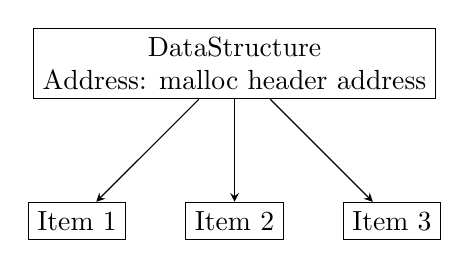
\begin{tikzpicture}[>=stealth, every node/.style={shape=rectangle, draw, align=center}]
            % Nodes
            \node (root) at (0,0) {DataStructure\\Address: malloc header address};
            \node (item1) at (-2,-2) {Item 1};
            \node (item2) at (0,-2) {Item 2};
            \node (item3) at (2,-2) {Item 3};
            % Edges
            \draw[->] (root) -- (item1);
            \draw[->] (root) -- (item2);
            \draw[->] (root) -- (item3);
        \end{tikzpicture}
        \caption{Graphical representation of an \texttt{rdf:Bag} container.}
    \end{figure}

    This small example illustrate how we can represent a container, or a relationship of belonging, using a graph. This is a concept that will be used later in the memory modelization process.

    \subsubsection{Inductive Reasoning and Learning}
    Inductive reasoning in Knowledge Graphs (KGs) involves techniques like embedding and Graph Convolutional Networks (GCNs) to learn the potential underlying structure of the graph. This is particularly useful for tasks like link prediction, node classification, and clustering.

    For the sake of clarity and grouping, we will present the concepts of graph embedding and GCNs in the next sections, but it is important to note that they are not mutually exclusive. In fact, GCNs can be used to generate embeddings, and embeddings can be used as input for GCNs. As such, they are often used together in the context of KGs, or in our case, memory graphs.

\section{Data preprocessing for Machine Learning}\label{sec:background:processing}
    \acrfull{ml} is a subfield of \acrfull{ai} that focuses on the development of algorithms that can learn from data and make predictions. It is a powerful tool that has been used to solve a wide range of problems, including image classification, speech recognition, and natural language processing. Before we can apply machine learning algorithms to a dataset, we must first prepare the data by performing various preprocessing steps. In this section, we will discuss the most common data preprocessing techniques, including data cleaning, feature engineering, and dataset splitting, as well as the importance of feature selection and dimensionality reduction. All those elements are crucial for the development of effective machine learning models for key extraction.

    \subsection{Feature engineering}
    In the realm of machine learning and data science, \textit{features} refer to individual measurable attributes or characteristics of the phenomena under study. Those features can be of different types, and can be used to predict the value of a target variable. 
    
    \subsubsection{Types of Features}
    Features can be of different types, depending on the nature of the data. The type of feature determines how it is processed and utilized by the model. The most common types of features include:

    \begin{itemize}
        \item \textbf{Numerical Features}: These are quantitative attributes representing measurements like height, weight, or age.
        \item \textbf{Categorical Features}: These are qualitative attributes representing discrete classes or labels, such as gender (Male, Female) or educational level (High School, Bachelor's, Master's).
        \item \textbf{Ordinal Features}: Similar to categorical features but with an inherent order, like ratings on a scale of 1 to 5.
        \item \textbf{Text Features}: These contain textual data and often require special preprocessing steps like tokenization and vectorization.
        \item \textbf{Temporal Features}: These are time-based attributes, such as timestamps, requiring special handling to capture time-dependent patterns.
        \item \textbf{Geospatial Features}: These attributes represent geographical or spatial coordinates.
    \end{itemize}

    Features are pivotal for the performance of machine learning models. The quality and pertinence of features can significantly influence the model's capability to discern underlying patterns in the data. Inadequately chosen or irrelevant features can lead to a poorly performing model, while carefully selected, relevant features can result in a robust and accurate model.

    \subsubsection{The Curse of Dimensionality}
    The \textit{curse of dimensionality} refers to a set of challenges that arise when dealing with high-dimensional data. As the number of features, or dimensions, in a dataset increases, the volume of the feature space grows exponentially. This exponential growth leads to several issues:

    \begin{itemize}
        \item \textbf{Data Sparsity}: In high-dimensional spaces, data points tend to be sparse, making it difficult for algorithms to identify patterns. The sparsity also means that the notion of "distance" becomes less meaningful, which is problematic for algorithms that rely on distance metrics.
        
        \item \textbf{Computational Complexity}: The exponential increase in volume demands significantly more computational power and memory, making it challenging to process and analyze the data efficiently.
        
        \item \textbf{Overfitting}: High dimensionality increases the risk of overfitting, where a model learns the noise in the data rather than the actual pattern. Overfit models perform poorly on unseen data.
        
        \item \textbf{Statistical Significance}: As dimensions increase, the amount of data required to achieve statistical significance also increases exponentially, often making it impractical to collect sufficient data.
        
        \item \textbf{Visualization and Interpretability}: High-dimensional data are difficult to visualize and interpret, making it challenging to derive intuitive insights.
    \end{itemize}

    Due to these challenges, many dimensionality reduction techniques have been developed to transform high-dimensional data into a lower-dimensional form, aiming to preserve as much of the relevant information as possible. These techniques are discussed in the next section.

    \subsubsection{Feature Engineering techniques}
    The meticulous process of selecting the most relevant features, or constructing new features from existing ones, is known as \textit{feature engineering}. This step can encompass normalization, transformation, and the creation of interaction terms among features. This complex process requires a deep understanding of the domain of study and the datasets, and is often a crucial step in the development of machine learning models \cite{FeatureEngineeringMadeEasy18}.

    In the context of \acrlong{ml}, features essentially serve as the input variables $ X $ that a machine learning model employs to make predictions or inferences about the output variable $ Y $. But not all features are equally informative. Some features may be redundant, irrelevant, or even detrimental to the model's performance. Irrelevant features are those that do not contribute to the predictive power of the model, while redundant features are those that are highly correlated with other features. Feature engineering techniques, can be used to build, transform or eliminate features, thereby reducing the dimensionality of the data and enhancing model performance \cite{FeatureSelecExtract14}.

    \begin{itemize}
        \item \textbf{Scaling and Normalization:} Scaling and normalization are techniques used to transform the features to a similar scale. This is particularly important for algorithms that rely on distance metrics, such as \acrfull{knn} and \acrfull{svm}. Scaling and normalization can also help accelerate the training process by reducing the number of iterations required for the model to converge. Some common techniques include min-max scaling, z-score normalization, and log transformation.
        
        \item \textbf{Feature Extraction}: This technique involves transforming the original set of features into a new set of features, which is usually of lower dimensionality. The new features are often combinations of the original features and aim to capture as much of the information in the original data as possible. Many methods exit, like \acrfull{pca}, \acrfull{lda} and \acrfull{tsne} are often employed to transform high-dimensional data into a lower-dimensional form are commonly used for feature extraction \cite{FeatureSelecExtract14}.
        
        \item \textbf{Feature Selection}: Unlike feature extraction, feature selection aims to pick a subset of the most important features from the original set, without changing them \cite{FeatureSelecExtract14}. The goal is to remove irrelevant or redundant features that do not contribute significantly to the model's performance. Techniques like Recursive Feature Elimination (RFE) and using importance scores from tree-based algorithms like Random Forest are popular methods for feature selection.
    \end{itemize}

    Both techniques have their own advantages and disadvantages, and the choice between the two often depends on the specific requirements of the task at hand. Feature extraction is generally more suitable when the original features do not have much interpretability to begin with, or when transforming features can lead to a more compact and effective representation. On the other hand, feature selection is often preferred when it is important to maintain the interpretability of the features, or when computational efficiency is a concern \cite{FeatureEngineeringMadeEasy18}.

    \subsubsection{Evaluating Features with Correlation Tests}
    To assess the quality of features, various statistical measures can be employed. Correlation tests are statistical tests that measure the strength and direction of the relationship between two variables. Pearson, Kendall, and Spearman correlation coefficients are commonly used to quantify the linear or monotonic relationship between each feature and the target variable \cite{StatisticalMethodsInPractice09}. A high absolute value indicates a strong relationship, aiding in feature selection.

    \begin{itemize}
        \item \textbf{Pearson Correlation}: Measures the linear relationship between two variables. It ranges from -1 to 1, where -1 indicates a strong negative linear correlation, 1 indicates a strong positive linear correlation, and 0 indicates no linear correlation.
        \item \textbf{Kendall's Tau}: A non-parametric test that measures the strength and direction of a monotonic relationship between two variables.
        \item \textbf{Spearman's Rank}: Also a non-parametric test, it assesses how well an arbitrary monotonic function can describe the relationship between two variables without making any assumptions about the frequency distribution.
    \end{itemize}

    These techniques are useful for evaluating the relationship between each feature and allows to generate correlation matrices, which can be used to identify redundant features. It's also possible to evaluate each feature independently through univariate feature selection techniques. In Python's scikit-learn library \cite{ScikitLearn}, methods like \textit{F-test} and the \textit{p-value} are often used for this purpose.
"
    \begin{itemize}
        \item \textbf{F-test value}: Measures the linear dependency between the feature variable and the target. A higher F-test value indicates a more useful feature.
        \item \textbf{p-value}: Indicates the probability of an F-test value this large arising if the null hypothesis is true. A smaller p-value suggests rejecting the null hypothesis, making the feature significant.
    \end{itemize}

    In summary, features are the foundational elements of any machine learning model. The quality of these features, along with how they are processed and utilized, can markedly impact the model's performance. The significance of feature engineering cannot be overstated. Properly engineered features can drastically reduce modeling errors, leading to more accurate and reliable predictions. It serves as a bridge between raw data and predictive models, ensuring that the models are fed with the most relevant and informative features.

    \subsection{Embeddings}
    Embeddings are low-dimensional vector representations of high-dimensional objects. They are often used to capture complex relationships between objects and are particularly useful for machine learning tasks like clustering, classification, and link prediction. Embeddings are widely used in the field of natural language processing (NLP) to represent words, sentences, and documents \cite{UnderstandingWordEmbeddingsAndLM20}. In recent years, they have also been applied to graphs to learn node representations \cite{KG21}. In this section, we will discuss the concept of embeddings and explore some common techniques for creating them.
    
    \subsubsection{Embedding Creation vs Feature Engineering}    
    Both embedding creation and feature engineering are techniques used to transform data for machine learning models. However, they are different in terms of their goals and how they are achieved.

    \begin{itemize}
        \item \textbf{Embedding Creation}: Embedding creation is the process of learning a low-dimensional vector representation of a high-dimensional object. This involves mapping discrete objects, such as words in \acrfull{nlp} or nodes in a graph in our case, to vectors of continuous values in a lower-dimensional space \cite{UnderstandingWordEmbeddingsAndLM20}. The goal is to capture the semantic or structural relationships between these objects. Specialized algorithms like Word2Vec for word embeddings or Node2Vec for graph embeddings are often used.
        
        \item \textbf{Feature Engineering}: As discussed before, it is a more general practice that involves creating new features or modifying existing ones to improve the performance of a machine learning model. While feature engineering can include creating embeddings, it also encompasses a wide range of other techniques like normalization, transformation, outlier detection, and handling missing values.
    \end{itemize}

    In general, feature engineering is a more manual process, while embedding creation is more automated. Feature engineering requires domain knowledge and understanding of the problem, while embedding creation can be done using a variety of machine learning techniques.

    Thus, embedding creation is a specialized form of feature engineering aimed at mapping discrete objects to continuous vectors of numbers, usually for capturing complex relationships. Feature engineering, on the other hand, is a broader practice that can involve a variety of techniques, including but not limited to embedding creation.

    \subsubsection{Embeddings for graphs}\label{sec:background:processing:embedding:graph}
    Graph embedding techniques aim to map nodes and edges in a graph to vectors in a low-dimensional space \cite{KG21}. The primary goal is to preserve the graph's structural properties, such as node connectivity and community structure, in the embedded space. These vectors can then be used for various machine learning tasks like clustering, classification, and link prediction. A quite complete overwiew of the different techniques can be found in \citetitle{KG21}. Here are some common and advanced techniques:

    % need to complete this section with more details and references

    \paragraph{Translational Models}
    The first type of graph embeddings techniques is based around using transactional models that interpret edge labels as transformations from subject nodes to object nodes \citetitle{KG21}. 

    \begin{itemize}
        \item \textbf{TransE:} is one of the earliest and most straightforward translational models. It represents entities as points in a vector space and relations as translations between these points. The primary idea is that for a valid triple \((h, r, t)\), the equation \(h + r = t\) should hold, where \( h \) stands for the head entity, \( r \) represents the relation, and \( t \) is the tail entity. This model is simple and computationally efficient but is limited in its ability to capture complex relationships \cite{KG21}.
        \item \textbf{TransH:} TransH extends TransE by introducing relation-specific hyperplanes. This allows the model to capture more complex relationships by projecting the entity embeddings onto these hyperplanes before performing translations \cite{KG21}.
        \item \textbf{TransR:} TransR goes a step further by not only introducing relation-specific hyperplanes but also relation-specific translations. This allows for a more flexible representation of relations, accommodating various types of complexities \cite{KG21}.
        \item Other improvements include \textit{TransD} or \textit{MuRP}, which shows that research in this domain is still very active.
    \end{itemize}

    \paragraph{Tensor Decomposition Models}
    Tensor decomposition models represent entities and relations as vectors or matrices in a low-dimensional space. These models are based on the assumption that the relationship between entities can be represented by a bilinear function. They are computationally efficient and can capture complex relationships, but they are also limited in their ability to model asymmetric and reflexive relations.

    \begin{itemize}
        \item \textbf{RESCAL:} RESCAL employs a bilinear model where each relation is represented by a full-rank matrix. This allows for capturing asymmetric and reflexive relations but at the cost of increased computational complexity \cite{KG21}.
        \item \textbf{DistMult:} DistMult simplifies RESCAL by assuming that the relation matrices are diagonal. This reduces the number of parameters and computational complexity, making it more scalable \cite{KG21} \cite{KG22}.
        \item \textbf{ComplEx:} ComplEx extends DistMult by introducing complex-valued embeddings. This allows the model to capture asymmetric relations effectively while maintaining computational efficiency \cite{KG21} \cite{KG22}.
    \end{itemize}

    \paragraph{Neural Models}
    Neural models employ neural networks to learn the features of entities and relations. This provides a more flexible and adaptive approach to graph embeddings.

    \begin{itemize}
        \item \textbf{ConvKB:} ConvKB employs a convolutional neural network to automatically learn the features of entities and relations. It is technical a translational model as introduced before, but uses a convolutional layer to capture the interactions between entities and relations. This provides a more flexible and adaptive approach to graph embeddings \cite{ConvKB18}.
        \item \textbf{RotatE:} RotatE uses complex rotations in the embedding space to model relations. This neural model captures the semantics of relations in a more expressive manner \cite{KG22}.
        \item \textbf{SDNE (Structural Deep Network Embedding)}: SDNE employs a deep autoencoder to learn complex and non-linear node embeddings while preserving first-order and second-order proximities. It is particularly effective for capturing intricate patterns and structures in the graph \cite{SDNE16}.
        \item \textbf{R-GCN:} Relational Graph Convolutional Networks (R-GCNs) combine the strengths of GCNs and traditional embedding methods to capture both topological and semantic information \cite{RGCN18}. A more recent study by \citeauthor{RGCN22} argues that the main contribution of R-GCN lies in its message passing paradigm rather than the learned weights. This paper introduces a variant called Random R-GCN (RR-GCN) \cite{RGCN22}.
        \item \textbf{ConvE:} ConvE employs convolutional layers to capture local and global interactions between entities and relations, offering a more expressive representation \cite{KG22}.
    \end{itemize}

    \paragraph{Language Models}
    Language models utilize pre-trained language models to enrich the embeddings with contextual information. This approach leverages the recent developments of language models to capture the semantics of entities and relations.

    \begin{itemize}
        \item \textbf{BERT for KGE:} Utilizing pre-trained BERT models, this approach leverages the power of language models to enrich the embeddings with contextual information \cite{KGBERT19}.
        \item \textbf{BART KGE:} Bidirectional and Auto-Regressive Transformers (BART) is a denoising autoencoder that can be used for various NLP tasks. This approach utilizes BART to learn entity and relation embeddings. The paper introducing this also compares other \acrshort{llm} like GPT-2 \cite{KGBART21}.
        \item Due to the recent developments in NLP, this domain is still very active, and new approaches are being developed regularly.
    \end{itemize}

    \subsubsection{Word Embeddings}
    Word embeddings are vector representations of words in a low-dimensional space. They are often used as input for machine learning models in natural language processing (NLP) tasks like text classification, sentiment analysis, and machine translation. Word embeddings are typically learned from large text corpora using unsupervised learning techniques like Word2Vec and GloVe. These embeddings can then be used to capture semantic relationships between words and phrases, which is particularly useful for NLP tasks \cite{UnderstandingWordEmbeddingsAndLM20}.

    \begin{itemize}
        \item \textbf{Word2Vec}: Word2Vec is a popular algorithm for learning word embeddings from text data. It employs a shallow neural network to learn the embeddings and is often used as a pre-processing step for NLP tasks \cite{KG22}.
        \item \textbf{GloVe}: Global Vectors for Word Representation (GloVe) is another popular algorithm for learning word embeddings. It is based on the co-occurrence matrix of words and utilizes matrix factorization to learn the embeddings \cite{KG22}.
    \end{itemize}

    \paragraph{Graph Embeddings}
    Graph embeddings are vector representations of nodes in a graph.Graph embeddings are typically learned using unsupervised learning techniques like Node2Vec and DeepWalk. These embeddings can then be used to capture structural relationships between nodes, which is particularly useful for graph analytics tasks \cite{KG21}.
    
    \begin{itemize}
        \item \textbf{One-Hot Encoding}: This is a simple technique that represents each node as a vector of 0s and 1s, where the length of the vector is equal to the number of nodes in the graph. The vector contains a 1 at the index corresponding to the node and 0s everywhere else. As is, this method is not really suitable for large graphs as it results in a high-dimensional and sparse matrix representation \cite{KG22}.
        
        \item \textbf{Node2Vec}: This algorithm learns continuous feature representations for nodes by optimizing a neighborhood-preserving objective. It employs biased random walks and uses the Skip-gram model to generate embeddings. Node2Vec is particularly effective for capturing local structures and can be fine-tuned for specific tasks \cite{Node2vec16}.
        
        \item \textbf{DeepWalk}: Similar to Node2Vec, DeepWalk uses random walks to generate node sequences. It employs the Skip-gram model from natural language processing to learn embeddings. Unlike Node2Vec, it does not use biased walks, making it more suitable for capturing global structures \cite{Deepwalk14}.
        
        \item \textbf{Spectral Clustering}: This technique is based on the spectral theory of graphs. It utilizes the eigenvalues and eigenvectors of the Laplacian matrix of the graph to find an optimal embedding. Spectral Clustering is particularly useful for community detection and can capture the global structure of the graph \cite{SpectralNetworks13} \cite{SemiSupervisedClassificationSpectralConvGCN16}.
        
        \item \textbf{LINE}: Large-scale Information Network Embedding (LINE) aims to preserve both local and global network structures. It optimizes two objectives: first-order and second-order proximities between nodes. LINE is scalable and can handle large graphs efficiently \cite{LINEEmbedding15}.
        
        \item \textbf{Graph Factorization}: This method directly factorizes the adjacency matrix of the graph to learn node embeddings, making it computationally efficient but less capable of capturing complex structures. It is often used for large-scale graphs where computational resources are limited \cite{KG22}.
        
    \end{itemize}

    \subsection{Other preprocessing techniques for Machine Learning}
    When working with real-world data and datasets, it is common to issues like missing values, outliers, and imbalanced classes that can adversely affect the performance of machine learning models. In this section, we will discuss some common preprocessing techniques used to improve the quality of data and ensure that the models can learn effectively.

    \subsubsection{Data Cleaning}
    Data cleaning is the process of detecting and correcting errors in the data. It is a crucial step in data preprocessing and involves various techniques like outlier detection, handling missing values, and data normalization. Data cleaning is necessary to ensure that the data is accurate and consistent, which is essential for machine learning models to learn effectively.

    \begin{itemize}
        \item \textbf{Outlier Detection}: Outliers are data points that deviate significantly from the rest of the dataset. They can be caused by errors in data collection or genuine variations. Outliers can skew the model's learning and should be identified and handled appropriately, either by removal or transformation.
        
        \item \textbf{Handling Missing Values}: Missing data can lead to biased or incorrect model training. Techniques for handling missing values include imputation, where missing values are replaced with statistical measures like mean, median, or mode, and deletion, where rows with missing values are removed.
        
        \item \textbf{Data Normalization}: Features with different scales can affect the performance of machine learning algorithms. Normalization rescales the features to a standard range, usually [0, 1], or transforms them to have a mean of 0 and a standard deviation of 1.
        
        \item \textbf{Encoding Categorical Variables}: Many machine learning algorithms require numerical input and output variables. Categorical variables are converted to numerical format through techniques like one-hot encoding or label encoding.
        
        \item \textbf{Text Cleaning}: In natural language processing tasks, text data may require cleaning to remove irrelevant characters, correct typos, or standardize text format.
        
        \item \textbf{Duplicate Removal}: Duplicate entries can bias the model and should be identified and removed from the dataset.
        
        \item \textbf{Feature Engineering}: While not strictly data cleaning, feature engineering involves transforming existing features or creating new ones to improve model performance.
    \end{itemize}

    \subsubsection{Dataset splitting and sampling}
    One other typical step is the division of the dataset into training and testing sets. This separation is crucial for evaluating the generalization performance of a model. The training set is used to train the model, while the testing set is used to evaluate its performance on unseen data. Failing to separate these sets can lead to overfitting, where the model performs well on the training data but poorly on new, unseen data.

    Various techniques exist for dataset splitting and sampling, each with its own advantages and disadvantages:

    \begin{itemize}
        \item \textbf{Random Split}: The dataset is randomly divided into training and testing sets based on a given ratio, such as 70\% for training and 30\% for testing. This method is simple but may result in imbalanced classes in the splits.
        
        \item \textbf{Stratified Split}: Similar to random split, but ensures that the distribution of classes is the same in both training and testing sets. This is particularly useful for imbalanced datasets.
        
        \item \textbf{k-Fold Cross-Validation}: The dataset is divided into 'k' subsets or "folds." The model is trained on k-1 folds and tested on the remaining fold. This process is repeated k times, each time with a different fold as the testing set. The average performance metric is used for evaluation.
        
        \item \textbf{Leave-One-Out Cross-Validation (LOOCV)}: A special case of k-Fold Cross-Validation where k is equal to the number of data points. Each data point is used once as the test set while the remaining points form the training set.
        
        \item \textbf{Bootstrapping}: Random samples are drawn with replacement from the dataset to create multiple training sets. The model is trained and tested on these sets, and the average performance is calculated.
    \end{itemize}

    \subsubsection{Dealing with Imbalanced Datasets}
    Imbalanced datasets are those where the classes are not represented equally. This is a common issue in machine learning, especially in classification problems. An imbalanced dataset can lead to a biased model that may not effectively predict the minority class. Therefore, it is crucial to address this issue during data preprocessing.

    \begin{itemize}
        \item \textbf{Why it is Necessary}: In imbalanced datasets, machine learning algorithms tend to be biased towards the majority class, ignoring the minority class. This results in poor classification performance for the minority class, which is often the class of interest in problems like fraud detection, medical diagnosis, etc.
        
        \item \textbf{Oversampling}: This involves adding more copies of the minority class. Oversampling can be random with replacement, or it can involve generating synthetic samples.
        
        \item \textbf{Undersampling}: This involves removing some of the samples of the majority class. This method is generally not preferred as it can lead to loss of data.
        
        \item \textbf{SMOTE (Synthetic Minority Over-sampling Technique)}: SMOTE is an oversampling method that creates synthetic samples in the feature space. It selects two or more similar instances (using a distance measure) and perturbing an instance one at a time by a random amount within the difference to the neighboring instances.
        
        \item \textbf{ADASYN (Adaptive Synthetic Sampling)}: Similar to SMOTE, but it uses a weighted distribution for different minority class examples according to their level of difficulty in learning. 
        
        \item \textbf{Cost-sensitive Learning}: This involves modifying the algorithm to increase the weight of the minority class during training, thereby making the algorithm more sensitive to it.
        
        \item \textbf{Ensemble Methods}: Methods like Random Forest and Gradient Boosting can be used with techniques like bagging and boosting to handle imbalanced datasets effectively.
        
        \item \textbf{Resampling Methods}: These involve randomly partitioning the data into subsets, balancing each subset, and then aggregating the results.
    \end{itemize}

    To conclude this section, data preprocessing is a crucial step in machine learning. The number of concepts and techniques discussed here is by no means exhaustive, which further highlights the importance and complexity of data preprocessing. 

\section{Machine Learning and Deep Learning}\label{sec:background:ml}
    In the preceding sections, we have discussed the importance of data preprocessing and feature engineering for machine learning. In this section, we will discuss the machine learning pipeline and explore some common machine learning algorithms. We will also discuss deep learning and neural networks especially in the context of graphs, since they have gained popularity in recent years due to their superior performance on many tasks.

    \subsection{Machine Learning}
    Machine learning is a cornerstone in the field of artificial intelligence and has been instrumental in driving many of today's technological and scientific breakthroughs. From natural language processing to computer vision, machine learning algorithms play a critical role in making sense of large and complex data sets.

        \subsubsection{What is Machine Learning}
        Machine learning is a subfield of artificial intelligence that provides systems the ability to automatically learn and improve from experience without being explicitly programmed. This learning process is based on the recognition of complex patterns in data and the making of intelligent decisions based on them \cite{ScienceMachineLearning15}.

        The machine learning pipeline typically involves several steps including some pre-steps like data collection, preprocessing, feature extraction that we have already discussed before, usually followed by model training, evaluation, and deployment. Algorithms are trained on a dataset, and the learned patterns are used to make predictions or decisions without human intervention. \acrshort{ml} algorithms can be broadly classified into three categories \cite{ScienceMachineLearning15}:

        \begin{itemize}
            \item \textbf{Supervised Learning}: Algorithms are trained on labeled data, and the aim is to make predictions or map inputs to outputs.
            \item \textbf{Unsupervised Learning}: Algorithms are trained on unlabeled data, focusing on the underlying structure or distribution in the data.
            \item \textbf{Reinforcement Learning}: Algorithms learn to perform an action from state to state to maximize some type of reward or objective function.
        \end{itemize}

        In the following, we will focus on supervised and unsupervised learning, as they are the most relevant to our work.

        \subsubsection{Model Evaluation}
        Evaluating the performance of a machine learning model is crucial for understanding its effectiveness and suitability for a given task. It is not a trivial task as it depends on various factors like the type of data, the problem at hand, and the model itself \cite{EvaluatingQualityMLExplanations21}. In this section, we will discuss some common evaluation metrics for classification and regression models.
    
        \begin{minipage}{\dimexpr\linewidth-20pt}
            \paragraph{Precision}
            Precision is the ratio of correctly predicted positive observations to the total predicted positives. The formula for precision is:
            \par
            \vspace{2em}
            \begin{center}
                $
                \text{Precision} = \frac{\text{True Positives}}{\text{True Positives} + \text{False Positives}}
                $
            \end{center}
            \vspace{1em}
        \end{minipage}
    
        \begin{minipage}{\dimexpr\linewidth-20pt}
            \paragraph{Recall}
            Recall is the ratio of correctly predicted positive observations to all the observations in the actual class. The formula for recall is:
            \par
            \vspace{2em}
            \begin{center}
                $
                \text{Recall} = \frac{\text{True Positives}}{\text{True Positives} + \text{False Negatives}}
                $
            \end{center}
            \vspace{1em}
        \end{minipage}
    
        \begin{minipage}{\dimexpr\linewidth-20pt}
            \paragraph{F-1 Score}
            The F-1 Score is the weighted average of Precision and Recall, and it ranges from 0 to 1. The formula for the F-1 Score is:
            \par
            \vspace{2em}
            \begin{center}
                $
                \text{F-1 Score} = 2 \times \frac{\text{Precision} \times \text{Recall}}{\text{Precision} + \text{Recall}}
                $
            \end{center}
            \vspace{1em}
        \end{minipage}
    
        \begin{minipage}{\dimexpr\linewidth-20pt}
            \paragraph{Accuracy}
            Accuracy is the ratio of correctly predicted observations to the total observations. The formula for accuracy is:
            \par
            \vspace{2em}
            \begin{center}
                $
                \text{Accuracy} = \frac{\text{True Positives} + \text{True Negatives}}{\text{Total Observations}}
                $
            \end{center}
            \vspace{1em}
        \end{minipage}

        These are the most common metrics used for evaluating classification models. Other metrics like the Area Under the Curve (AUC) and the Receiver Operating Characteristic (ROC) curve are also used for evaluating binary classification models. For regression models, metrics like Mean Squared Error (MSE), Root Mean Squared Error (RMSE), and Mean Absolute Error (MAE) are commonly used \cite{ScikitLearn}.

        \subsection{Machine Learning Models for Binary Classification}
        Binary classification is a supervised learning task where the goal is to predict a binary outcome, i.e., one of two possible classes (0 or 1). This is a truly classical task for a \acrshort{ml} model, with a range of applicable algorithms. As such, we rely on Python's Scikit-learn library for implementation.

        \paragraph{Logistic Regression}
        A specialized form of regression tailored for predicting binary outcomes. It employs the logistic function to map predicted values between 0 and 1. While straightforward and interpretable, its performance may be limited on complex, non-linear data \cite{nick_logistic_2007}.

        \begin{minipage}{\dimexpr\linewidth-20pt}
            The logistic function is defined as:
            \par
            \vspace{2em}
            \begin{center}
                $
                P(y=1|x) = \frac{1}{1 + e^{-(\beta_0 + \beta_1 x)}}
                $
            \end{center}
            \vspace{1em}
            Where \( \beta_0 \) is the intercept and \( \beta_1 \) is the coefficient for the predictor variable \( x \).
        \end{minipage}

        \paragraph{Decision Trees}
        These are versatile models used for both classification and regression. They partition the feature space into regions, making decisions at each node. While easy to visualize, they are susceptible to overfitting \cite{kotsiantis_decision_2013}.

        \begin{minipage}{\dimexpr\linewidth-20pt}
            Decision Trees use metrics like Gini impurity or entropy to make splits:
            \par
            \vspace{2em}
            \begin{center}
                $
                \text{Gini}(T) = 1 - \sum_{i=1}^{C} p_i^2
                $
            \end{center}
            \vspace{1em}
            Where \( T \) is a node and \( p_i \) is the proportion of class \( i \) instances among the training instances in node \( T \).
        \end{minipage}

        \paragraph{Random Forest}
        An ensemble technique that aggregates predictions from multiple decision trees. Known for its robustness and ability to handle large, high-dimensional data \cite{probst_hyperparameters_2019}.

        \begin{minipage}{\dimexpr\linewidth-20pt}
            The final prediction is an average or majority vote from all trees:
            \par
            \vspace{2em}
            \begin{center}
                $
                \hat{y} = \frac{1}{n} \sum_{i=1}^{n} \hat{y_i}
                $
            \end{center}
            \vspace{1em}
            Where \( \hat{y} \) is the final prediction and \( \hat{y_i} \) is the prediction from the \( i^{th} \) tree.
        \end{minipage}

        \paragraph{Support Vector Machines (SVM)}
        Effective for both classification and regression, SVMs find the hyperplane that best separates the data into classes. They excel in high-dimensional spaces \cite{wu_analysis_2006}.

        \begin{minipage}{\dimexpr\linewidth-20pt}
            The objective is to maximize the margin between classes:
            \par
            \vspace{2em}
            \begin{center}
                $
                \max_{w, b} \frac{2}{\| w \|}
                $
            \end{center}
            \vspace{1em}
            Where \( w \) is the weight vector and \( b \) is the bias term.
        \end{minipage}

        \paragraph{k-Nearest Neighbors (k-NN)}
        An instance-based algorithm that classifies a new point based on the majority class among its 'k' nearest neighbors \cite{laaksonen_classification_1996}.

    \begin{minipage}{\dimexpr\linewidth-20pt}
        The distance between points is often calculated using Euclidean distance:
        \par
        \vspace{2em}
        \begin{center}
            $
            d(x, y) = \sqrt{\sum_{i=1}^{n} (x_i - y_i)^2}
            $
        \end{center}
        \vspace{1em}
        Where \( d(x, y) \) is the distance between points \( x \) and \( y \), and \( n \) is the number of dimensions.
    \end{minipage}

    \subsection{Deep Learning}
    Deep learning offers a powerful set of tools for automatically generating embeddings from the graph representation of heap dumps. Leveraging neural networks, we can build custom models using PyTorch to perform binary classification tasks, such as predicting key nodes in a heap dump. In this section, we will explore various neural network architectures that are well-suited for this task.

    Neural Networks serve as the backbone of deep learning models \cite{DeepLearningBook16}. They consist of interconnected nodes or "neurons" organized into layers. Deep learning extends this architecture by employing multiple hidden layers, enabling the model to learn complex representations from data. This is particularly useful when dealing with graph-based heap dump representations, where the relationships between nodes can be intricate \cite{KG22}. 
    
    Choosing Deep Learning models is dependent on the task. As such, we need to present the different types of neural networks and their advantages and disadvantages. Below are some common neural network architectures:

    \subsubsection{Recurrent Neural Networks (RNN)}
    \acrfull{rnn} are particularly effective for sequence-based data. In the context of heap dumps, if the memory addresses or keys exhibit some form of sequential pattern, RNNs can be employed to capture these temporal dependencies for binary classification \cite[10.2]{DeepLearningBook16}.

    \begin{itemize}
        \item \textbf{Advantages:}
        \begin{itemize}
            \item Good at capturing short-term dependencies in sequence data.
            \item Relatively simpler architecture.
        \end{itemize}
        \item \textbf{Disadvantages:}
        \begin{itemize}
            \item Struggles with long-term dependencies due to the vanishing gradient problem.
            \item May require more data for effective training.
        \end{itemize}
    \end{itemize}

    \subsubsection{Long Short-Term Memory (LSTM)}
    LSTMs are an extension of RNNs designed to capture long-term dependencies, making them suitable for more complex sequences \cite{hochreiter_long_1997}.

    \begin{itemize}
        \item \textbf{Advantages:}
        \begin{itemize}
            \item Effective in capturing long-term dependencies.
            \item Less susceptible to the vanishing gradient problem.
        \end{itemize}
        \item \textbf{Disadvantages:}
        \begin{itemize}
            \item More complex and computationally intensive than RNNs.
            \item May require fine-tuning of hyperparameters.
        \end{itemize}
    \end{itemize}

    \subsubsection{Gated Recurrent Units (GRU)}
    \acrfull{gru} offer a compromise between the simplicity of RNNs and the power of LSTMs. They are effective in capturing both short-term and long-term dependencies but with a less complex architecture \cite{chung_empirical_2014}.

    \begin{itemize}
        \item \textbf{Advantages:}
        \begin{itemize}
            \item Simpler architecture compared to LSTM.
            \item Efficient in capturing long-term dependencies.
        \end{itemize}
        \item \textbf{Disadvantages:}
        \begin{itemize}
            \item May not perform as well as LSTMs for very complex sequences.
            \item Still more computationally intensive than basic RNNs.
        \end{itemize}
    \end{itemize}

    \subsubsection{Convolutional Neural Networks (CNN)}
    Though traditionally used in image processing, CNNs can also be adapted for sequence data like heap dumps. They are excellent at identifying spatial hierarchies or patterns in the data \cite{DeepLearningBook16} \cite{lecun_gradient_based_1998}.

    \begin{itemize}
        \item \textbf{Advantages:}
        \begin{itemize}
            \item Highly effective in identifying local patterns.
            \item Less prone to overfitting due to pooling layers.
        \end{itemize}
        \item \textbf{Disadvantages:}
        \begin{itemize}
            \item May not capture global dependencies as effectively as RNNs or LSTMs.
            \item Requires a fixed-size input.
        \end{itemize}
    \end{itemize}

    \subsubsection{Graph Convolutional Networks (GCN)}
    Graph Convolutional Networks (GCNs) are a specialized form of neural networks designed to work directly with graphs \cite{KG22}. They are particularly useful for our task as they can automatically generate embeddings from the graph representation of heap dumps. These embeddings can then be used for binary classification to predict key nodes.

    \begin{itemize}
        \item \textbf{Advantages:}
        \begin{itemize}
            \item Capable of capturing both local and global graph structures.
            \item No need for manual feature extraction from graphs.
        \end{itemize}
        \item \textbf{Disadvantages:}
        \begin{itemize}
            \item May require fine-tuning and a well-defined graph structure.
            \item Computationally intensive for large graphs.
        \end{itemize}
    \end{itemize}

    Several Python libraries can be used to implement GCNs for our specific task. Some of the notable ones are PyTorch Geometric, Spektral, and DGL (Deep Graph Library). These libraries offer pre-built GCN layers and various utilities to facilitate the embedding and binary classification of heap dump graphs.

    \subsection{Graph Neural Networks}
    A \acrfull{gnn} constructs a neural network that mirrors the structure of the underlying data graph. In this architecture, nodes are linked according to their relationships in the data graph. The model is trained in a supervised fashion to map input features of nodes to their corresponding output features \cite{KG22}. These output features can either be manually annotated or sourced from a knowledge graph. 

    Unlike traditional knowledge graph embeddings, GNNs offer the advantage of end-to-end supervised learning tailored for specific tasks. 
    
    With a dataset of labeled examples, GNNs can classify individual nodes or even entire graphs. The challenge lies both in how to convert a given graph to a format that can be fed into a neural network (see \autoref{sec:background:processing:embedding:graph}) and how to design a neural network that can effectively learn from the graph data. Note that the distinction between the two is not always clear since two problems are often tackled together. As such, the present classification is not exhaustive and arbitrary, even though it is based on the literature and meta-analysis of the field, like \citetitle{KG22} \cite{KG22} and \citetitle{GNNComprehensiveSurvey20} \cite{GNNComprehensiveSurvey20}.
    
    \acrshort{gnn}s have been employed in various applications, ranging from traffic prediction, recommender systems, and software verification \cite{GNNComprehensiveSurvey20}. Remarkably, GNNs can also serve as substitutes for conventional graph algorithms. For instance, they have been used to identify central nodes in knowledge graphs through supervised learning \cite{KG22}. The following sections delve into two specific types of GNNs: Recursive GNNs and Convolutional GNNs.

    \subsubsection{Recursive Graph Neural Networks (RecGNNs)}
    Recursive Graph Neural Networks (RecGNNs) serve as the foundational approach to graph neural networks \cite{KG22}. The model operates by passing messages between neighboring nodes to recursively compute results. The framework learns the functions that generate the expected output based on a training set of labeled nodes. \citeauthor{GNN08} \cite{GNN08} proposed a seminal \acrshort{gnn} model that uses feature vectors for nodes and edges, along with state vectors for nodes. Two parametric functions, the transition function and the output function, are used to update the state vectors and compute the final output for nodes, respectively. These functions are applied recursively until a fixpoint is reached. The model is highly flexible and can be adapted in various ways, such as defining neighboring nodes differently or using distinct parameters for each node \cite{GNN08}.

    \paragraph{Learning Process in \acrshort{gnn}s}
    The learning process in GNNs can be divided into three steps: input computation, node state update, and output computation. These steps are repeated until a fixpoint is reached, and the final output is computed for each node. Essentially, this involves finding the optimal parameters $ w $ such as for $ \varphi_{w} $ to best approximate the data in the learning dataset $ \mathcal{L} $. 

    \begin{minipage}{\dimexpr\linewidth-20pt}
        The learning task can be formulated as the minimization of a quadratic cost function $ e_{w} $ through iterative gradient descent \cite{GNN08}:
        \par
        \vspace{2em}
        \begin{center}
            \[
            e_{w} = \sum_{i=1}^{p}\sum_{j=1}^{q_{i}}(t_{i,j}-\varphi_{w}(G_{i},n_{i,j}) )^2
            \]
        \end{center}
        \vspace{1em}
    \end{minipage}

    Where:
    \begin{itemize}
        \item \( \mathcal{G} \): The set of graphs.
        \item \( \mathcal{N} \): The subset of nodes.
        \item \( \mathcal{D} = \mathcal{G} \times \mathcal{N} \): The set of pairs of a graph and nodes.
        \item \( G_{i} = (N_{i},E_{i}) \in \mathcal{G} \): The graph.
        \item \( N_{i} \): The set of nodes in graph \( G_{i} \).
        \item \( E_{i} \): The set of edges in graph \( G_{i} \).
        \item \( n_{i,j} \in N_{i} \): The \( j^{th} \) node of the graph \( G_{i} \).
        \item \( q_{i} \leq |N_{i}| \): The number of supervised nodes in the graph \( G_{i} \).
        \item \( p \leq |\mathcal{G}| \): The number of graphs in the learning set.
        \item \( \mathcal{L} = \{(G_{i},n_{i,j},t_{i,j})\} \): The learning set.
        \item \( t_{i,j} \in \mathbb{R}^m \): The target output for node \( n_{i,j} \).
        \item \( m \): The number of outputs.
        \item \( \mathbb{R}^m \): The \( m \)-dimensional Euclidean space.
        \item \( \varphi_{w} : \mathcal{D} \to \mathbb{R}^m \): The function that maps the input to the output.
        \item \( e_{w} \): Error function.
    \end{itemize}

    For graph-focused tasks, a special node is used for the target (\( t \)), whereas for node-focused tasks, supervision can be performed on every node. More information about the learning process can be found in \cite{GNN08}.

    \subsubsection{Convolutional Graph Neural Networks (ConvGNNs)}
    As introduced before, Graph Convolutional Networks extend the concept of convolution from images to graphs. \say{The core idea in the image setting is to apply small kernels (aka filters) over localised regions of an image using a convolution operator to extract features from that local region.} \cite{KG22}. They are designed to work with non-Euclidean data and are particularly useful for semi-supervised learning tasks on graphs. GCNs aim to learn a function that maps nodes to a low-dimensional space while considering their local neighborhood and features.

    \paragraph{Convolution filters}
    A Convolutional Neural Network (CNN) is a type of neural network that uses convolutional filters to extract features from images. These filters are applied to local regions of the image to capture spatial patterns \cite{CNNIntro15}. The same concept can be extended to graphs, where the convolution filters are applied to local regions of the graph to capture structural patterns. 

    \begin{minipage}{\dimexpr\linewidth-20pt}
        The convolution operation on an image is historically defined as follows \cite{ImageConvolution13} \cite{TutorialDeepLearningPart2}:
        \par
        \vspace{2em}
        \begin{center}
            \[
            y_{i,j} = \sum_{k=-m}^{m} \sum_{l=-n}^{n} x_{i+k,j+l} \times w_{kl}
            \]
        \end{center}
        \vspace{1em}
    \end{minipage}

    Where:
    \begin{itemize}
        \item \( y_{i,j} \): The output value at the coordinate $ (i,j) $ of the convolution output.
        \item \( x_{i,j} \): The input value at the coordinate $ (i,j) $ of the input image.
        \item \( w_{kl} \): The weight value (coefficient) of the kernel at the coordinate $ (k,l) $.
        \item \( m \): The kernel width.
        \item \( n \): The kernel height.
    \end{itemize}
    
    Similar to this, ConvGNNs implement the transition function using convolutions. One of the challenges in ConvGNNs is defining regions of a graph, as nodes in a graph may have varying numbers of neighbors. Solutions to this problem involve using spectral or spatial representations of graphs \cite{SemiSupervisedClassificationSpectralConvGCN16} \cite{KG22}. An alternative approach employs attention mechanisms to learn the most important features \cite{GAT17}. Unlike RecGNNs, ConvGNNs apply a fixed number of convolutional layers and can use different kernels/weights at each distinct step.

    % TODO: Give more details about doing convolutions on graphs

    Here are some common ConvGNN architectures. I recommend reading \citetitle{GCNAutoFiltering22} \cite{GCNAutoFiltering22} for a more in-depth discussion of these models:

    \begin{itemize}
        \item \textbf{Vanilla GCN}: The basic GCN model consists of an input layer, one or more hidden layers, and an output layer. Each layer is associated with a graph convolution operation that updates the node features based on their neighbors \cite{KG22}.
        
        \item \textbf{GraphSAGE (Graph Sample and Aggregation)}: This model generalizes the GCN framework by allowing various aggregation functions like mean, LSTM, and pooling to combine information from a node's neighbors \cite{GraphSAGE17}.
        
        \item \textbf{ChebNet}: ChebNet uses Chebyshev polynomials to generalize the convolution operation in the spectral domain. This allows the model to capture a broader range of graph structures \cite{GNNComprehensiveSurvey20}.
        
        \item \textbf{GAT (Graph Attention Networks)}: GAT introduces attention mechanisms into GCNs, enabling the model to weigh neighbors differently when aggregating information \cite{GAT17}.
        
        \item \textbf{MoNet}: This model employs a mixture model to generalize the convolution operation, making it capable of handling graphs with diverse structures \cite{MoNet17}.
        
        \item \textbf{Graph Isomorphism Network (GIN)}: GIN is designed to capture the isomorphism between different graphs, making it powerful for tasks like graph classification \cite{GCNAutoFiltering22}.
        
        \item Research on the topic is still ongoing, and a lot of new architectures are being proposed: Cluster-GCN, TAGCN, AutoGCN, and many more \cite{GCNAutoFiltering22}. It's worth noting that many of these models are not mutually exclusive and can be combined to create more powerful models.
    \end{itemize}

    The background chapter has introduced a lot of concepts and techniques that are relevant to our work. We have discussed the importance of data preprocessing and feature engineering, explored various machine learning algorithms, and looked at some common neural network architectures. Although not exhaustive, this overview should provide a solid foundation for the methods, design and implementation that will be discussed in the next chapters.
